\documentclass{beamer}
\usepackage[utf8]{inputenc}
\usepackage[T1]{fontenc}
\usepackage[english]{babel}
\usepackage[babel=true]{csquotes}
\usepackage{graphicx}
\usepackage[export]{adjustbox}
\usepackage{amsmath}
\usepackage{algorithm2e}
\usepackage{hyperref}
\usepackage{listings}
\usepackage[toc,page]{appendix}
\usepackage[backend=biber,style=alphabetic]{biblatex}


\graphicspath{ {../images/} }
\usetheme{Copenhagen}
\setbeamertemplate{page number in head/foot}[totalframenumber]


\title{Numerical stability ans fast-math}
\subtitle{Speeding up LHCb software through compilation optimization}
\author{Oscar Buon}


\begin{document}

\begin{frame}
    \centering
    \begin{minipage}{0.2\textwidth}
        
\includegraphics[width=\textwidth]{logo_ISIMA_INP.png}
    \end{minipage}\hfill
    \begin{minipage}{0.2\textwidth}
        
\includegraphics[width=\textwidth]{logo_CERN.png}
    \end{minipage}\hfill
    \begin{minipage}{0.2\textwidth}
        
\includegraphics[width=\textwidth]{logo_LHCb.png}
    \end{minipage}

    \maketitle

    Supervisor: Sebastien Ponce
\end{frame}

\part{Body}

\begin{frame}
    \frametitle{Table of contents}
    \tableofcontents
\end{frame}

\section{Introduction}

\begin{frame}
    \tableofcontents[currentsection]
\end{frame}

\subsection{Floating-point arithmetic}

\begin{frame}
    \frametitle{Floating-point arithmetic}

    \begin{displaymath}
        \begin{split}
            (0.75)_{10} & = (+ 7.5 \times 10^{-1})_{10} \\
            & = (\underbrace{+}_{sign} \underbrace{1.1}_{mantissa} \times 2^{\overbrace{-1}^{exponent}})_{2} = (0.11)_{2}
        \end{split}
    \end{displaymath}
\end{frame}

\subsection{IEEE 754}

\begin{frame}
    \frametitle{IEEE 754}

    \begin{itemize}
        \item 32 bits and 64 bits formats
        \item Subnormal numbers
        \item Special values: -Inf, +Inf, NaN
        \item Rounding rules
        \item Exception handling
        \item We should always consider floats as approximations !
    \end{itemize}
\end{frame}

\section{Correctness of some computes}

\begin{frame}
    \tableofcontents[currentsection]
\end{frame}

\subsection{Floats equality}

\begin{frame}[fragile]
    \frametitle{Floats equality}

    \begin{itemize}
        \item Never check for float equality.
        \item GCC flag \verb'-Wfloat-equal'.
              Ex. in LHCb:
              \begin{itemize}
                  \item \verb'0 == ip'
                  \item \verb'0.5 == ip'
                  \item \verb'lhs.m_energy == rhs.m_energy'
              \end{itemize}
    \end{itemize}
\end{frame}

\subsection{Exception cases}

\begin{frame}[fragile]
    \frametitle{Exception cases}

    \begin{lstlisting}[language=c++]
if (f(x) != 0.)
        return 5./f(x)
    \end{lstlisting}

    \begin{itemize}
        \item Maybe the two \verb'f(x)' will not be the sames.
    \end{itemize}
\end{frame}

\begin{frame}[fragile]
    \begin{lstlisting}[language=c++]
if ((float y = f(x)) != 0.)
        return 5./y
    \end{lstlisting}

    \begin{itemize}
        \item Maybe \verb'f(x)' will still be calculated twice.
        \item if \verb'f(x)' is close to $0$ then \verb'5./y' could be +Inf.
    \end{itemize}
\end{frame}

\begin{frame}[fragile]
    We should use:
    \begin{itemize}
        \item Using \verb'isfinite' after the compute.
    \end{itemize}

    There is also:
    \begin{itemize}
        \item The trapping system (registering a handler with \verb'signal()').
        \item The signaling system via \verb'std::numeric_limits<T>::signaling_NaN'.
    \end{itemize}
\end{frame}

\section{Fast-math}

\begin{frame}
    \tableofcontents[currentsection]
\end{frame}

\begin{frame}[fragile]
    \frametitle{Principle}

    \begin{itemize}
        \item Making mathematically valid optimizations but not respecting Standard.
        \item Different results but not more wrong than without \verb'fast-math'.
    \end{itemize}
\end{frame}

\subsection{Exception handling}

\begin{frame}[fragile]
    \frametitle{no-math-errno}

    \begin{itemize}
        \item Do not set \verb'errno' after calling math functions that are executed with a single instruction, e.g., \verb'sqrt'.
    \end{itemize}
\end{frame}

\begin{frame}[fragile]
    \frametitle{no-signaling-nans}

    \begin{itemize}
        \item Compile code assuming that IEEE signaling NaNs may not generate user-visible traps during floating-point operations.
        \item Enables optimizations that may change the number of exceptions visible with signaling NaNs.
        \item Enabled by default.
    \end{itemize}
\end{frame}

\begin{frame}[fragile]
    \frametitle{no-trapping-math}

    \begin{itemize}
        \item Compile code assuming that floating-point operations cannot generate user-visible traps.
              These traps include division by zero, overflow, underflow, inexact result and invalid operation.
        \item Implies no-signaling-nans.
    \end{itemize}
\end{frame}

\begin{frame}[fragile]
    \frametitle{finite-math-only}

    \begin{itemize}
        \item Allow optimizations for floating-point arithmetic that assume that arguments and results are not NaNs or +-Infs.
        \item Compiler can replace \verb'isnan' by \verb'false'.
              Actually it is an undefined behavior.
        \item Main source of bugs from \verb'fast-math'.
    \end{itemize}
\end{frame}

\subsection{Approximation}

\begin{frame}
    \frametitle{no-rounding-math}

    \begin{itemize}
        \item Round-to-zero for all floating point to integer conversions, and round-to-nearest for all other arithmetic truncations.
        \item Enabled by default.
    \end{itemize}
\end{frame}

\begin{frame}[fragile]
    \frametitle{no-signed-zeros}

    \begin{itemize}
        \item Allow optimizations for floating-point arithmetic that ignore the signedness of zero.
        \item Ex. \verb'0.0+x' or \verb'0.0*x'.
    \end{itemize}
\end{frame}

\begin{frame}[fragile]
    \frametitle{associative-math}

    \begin{itemize}
        \item Allow re-association of operands in series of floating-point operations.
        \item Can optimize \verb'2.0*x*3.0' in \verb'6.0*x' $\implies$ make some computes at compile time.
        \item May allow a better vectorization and use of \emph{FMA}.
        \item Needs no-signed-zeros and no-trapping-math.
    \end{itemize}
\end{frame}

\begin{frame}[fragile]
    \frametitle{reciprocal-math}

    \begin{itemize}
        \item Allow the reciprocal of a value to be used instead of dividing by the value if this enables optimizations.
        \item Ex. Replacing \verb'x/y' by \verb'x*(1/y)'.
        \item Decreases precision.
    \end{itemize}
\end{frame}

\begin{frame}[fragile]
    \frametitle{unsafe-math-optimizations}

    \begin{itemize}
        \item Allow optimizations for floating-point arithmetic that (a) assume that arguments and results are valid and (b) may violate IEEE or ANSI standards.
        \item When used at link time, it may include libraries or startup files that change the default FPU control word or other similar optimizations.
        \item Can affect dynamically included libraries.
        \item Enables -fno-signed-zeros, -fno-trapping-math, -fassociative-math and -freciprocal-math.
    \end{itemize}
\end{frame}

\section{Results}

\begin{frame}
    \tableofcontents[currentsection]
\end{frame}

\subsection{Improvement}

\begin{frame}[fragile]
    \frametitle{Improvement}

    Test: \verb'hlt2_pp_thor' ($2 \times 1000$ events)
    \begin{center}
        \begin{tabular}{ c c c }
            Optimization                                 & Improvement & Confidence interval ($2\sigma$) \\
            Fast-math\footnote{without finite-math-only} & $0\%$       & $\pm 0\%$                       \\
            Associative-math                             & $4.73\%$    & $\pm 0.87\%$                    \\
            Fast-math + LTO \& PGO                       & $12.04\%$   & $\pm 0.73\%$
        \end{tabular}
    \end{center}
\end{frame}

\begin{frame}[fragile]
    \frametitle{VTune}

    \begin{figure}[!htb]
        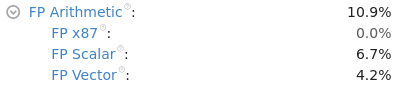
\includegraphics[width=0.5\textwidth, center]{reference_vtune.png}
        \caption{Reference}
    \end{figure}

    \begin{figure}[!htb]
        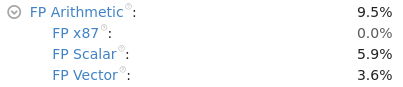
\includegraphics[width=0.5\textwidth, center]{associative-math_vtune.png}
        \caption{Associative-math}
    \end{figure}
\end{frame}

\subsection{Difference}

\begin{frame}[fragile]
    \frametitle{Difference}

    Difference with the reference (all counters):
    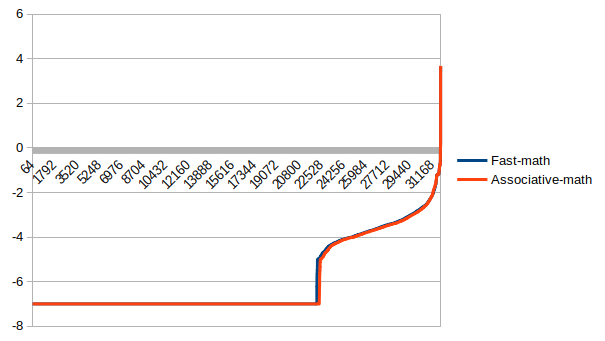
\includegraphics[width=\textwidth]{fast-math_difference.png}
\end{frame}

\part{Conclusion}

\begin{frame}[fragile]
    \frametitle{Conclusion}

    \begin{itemize}
        \item Enabling \verb'-Wfloat-equal'.
        \item Enabling fast-math at least for checking unstability.
        \item Other advantages:
              \begin{itemize}
                  \item Better precision in most cases (\emph{FMA} and \verb'double-precision-constant').
                  \item Coding clear equations and letting compiler optimize them.
                  \item GPU already using similar principles.
                  \item Make it clear that floats are approximations.
              \end{itemize}
    \end{itemize}
\end{frame}

\end{document}
